\documentclass[../CSC_52081_EP.tex]{subfiles}

\begin{document}
\section{Methodology / Approach}


\subsection{Environment and Agent Implementation}
\label{sec:CNN}

This study employs the CarRacing-v3 environment from Gymnasium \cite{gymnasium}, a challenging benchmark characterized by high-dimensional visual observations and multiple action modalities. In order to transform the observation space (a 3x96x96 picture frame) in the action space supported by the environment, we implemented a Convolutional Neural Network (CNN) inspired by \cite{DQN_CNN} with the following characteristics:

\begin{itemize}
    \item \textbf{Image}: the frames are transformed from an RGB state representation to grayscale, and the resolution is downscaled to 84x84 pixels. These steps facilitate the network computations, making them less complex. Additionally, to allow the network to accurately track the car's dynamics and improve the agent's ability to adjust actions based on the current state, each frame is stacked with the previous three frames. As a result, every state is represented by a sequence of four consecutive grayscale frames at 84x84 resolution (see Figure \ref{fig:grayscale}).

    \item \textbf{Input Layer}: 4-channel 84x84 images.

    \item \textbf{First Convolutional Layer}: 16 filters, 8x8 kernel, stride 4, ReLU activation. After applying the convolution, the output have dimensions 20x20.

    \item \textbf{Second Convolutional Layer}: 32 filters, 4x4 kernel, stride 2, ReLU activation. After applying the convolution, the output have dimensions 9x9.

    \item \textbf{Flatten Layer}: The output from the second convolutional layer is flattened into a 1D vector. The size of this vector is 32 * 9 * 9 = 2592.

    \item \textbf{First Fully Connected (FC) Layer}: 256 neurons, ReLU activation.

    \item \textbf{Second Fully Connected (FC) Layer}: The last fully connected layer defines the action space of the environment. For discrete action-space trials (DQN and Deep SARSA), this layer consists of five neurons with a linear activation function. In contrast, for continuous action-space tests (PPO, SAC, and CEM), the output layer comprises three neurons with different activation functions: \textit{tanh} for the steering action (ranging from [-1, 1]) and \textit{sigmoid} for the gas and brake actions (both ranging from [0, 1]).
\end{itemize}

\begin{figure}[H]
    \centering
    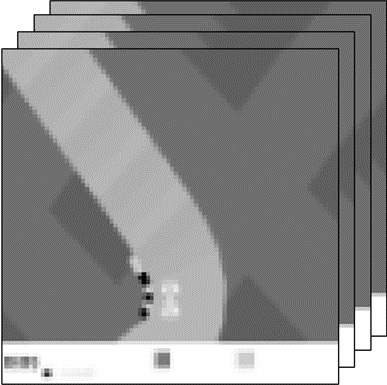
\includegraphics[scale = 0.3]{figures/grayscale_4.png}
    \caption{Input observation space for the CNN, composed by four grayscale consecutive frames from the car racing environment. Reference: \cite{DQN_CNN}}
    \label{fig:grayscale}
\end{figure}

\begin{figure}[H]
    \centering
    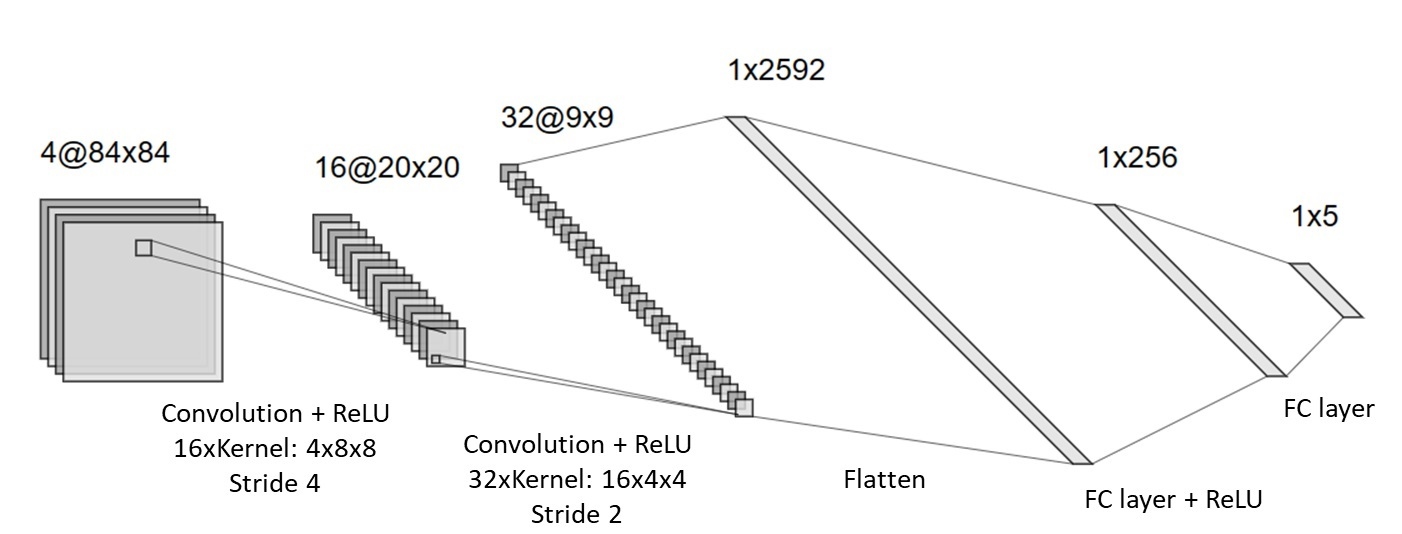
\includegraphics[scale = 0.15]{figures/CNN.png}
    \caption{Convolutional Neural Network (CNN) architecture for processing the observation from the car racing environment. Reference: \cite{DQN_CNN}}
    \label{fig:CNN}
\end{figure}

\subsection{Replay Buffer}
A key innovation introduced in the original DQN paper is the concept of experience replay. This technique involves storing experiences in a replay memory buffer, allowing the agent to break the temporal dependencies between consecutive experiences. During training, random minibatches are sampled from this buffer, which improves the stability of the learning process.

\subsection{Algorithms Design}

\hspace{1cm}

\subsubsection{DEEP Q-Network (DQN)}
The model is trained by optimizing a loss function based on the temporal difference error between predicted and target Q-values.

For the DQN, the target network consists in maintaining two separate networks: the main (or online) network, which is used for learning and selecting actions, and the target network, which is updated less frequently. The target network is a copy of the online network, and its parameters are periodically updated by copying the parameters of the online network to it. This approach helps stabilize the learning process by providing a fixed target for the updates, preventing oscillations and divergence in the Q-value estimates.

Training is conducted on minibatches of state-action-reward-next state sequences sampled from the replay buffer. The update rule of the algorithm is given by:
    \begin{equation}
        Q(s, a) \leftarrow Q(s, a) + \alpha \left[ r + \gamma \max_{a'} Q(s', a') - Q(s, a) \right]
    \end{equation}

    where $\max_{a'} Q(s', a')$ is the maximum Q-value at the next state $s'$ (greedy selection).

\hspace{1cm}

\subsubsection{DEEP SARSA}
For the SARSA algorithm, learning is performed using a single Q-network instead of maintaining a separate target network. The algorithm follows an on-policy approach, where the agent updates its Q-values based on the actions it actually takes, rather than using a target derived from the maximum possible future reward. This ensures that updates remain consistent with the agent’s current policy.

Training is conducted on minibatches of state-action-reward-next state-next action sequences sampled from the replay buffer. The update rule of the algorithm is given by:

\begin{equation}
        Q(s, a) \leftarrow Q(s, a) + \alpha \left[ r + \gamma Q(s', \pi(s')) - Q(s, a) \right]
    \end{equation}

where $Q(s', \pi(s'))$ corresponds to the Q-value of the next state-action pair, following the agent’s current policy ($\epsilon$-greedy). This approach ensures that the learning process accounts for the agent’s actual behavior, rather than assuming a greedy action selection at every step. $\epsilon$ is then decayed for better balance between prioritizing exploration at the beggining, and more exploitation after.

\hspace{1cm}

\subsubsection{Proximal Policy Optimization (PPO)}
The training for the PPO is described as follows:

\begin{itemize}
    \item First, we collect trajectories from the environment:
    \[
    \mathcal{D} = \{ (s_t, a_t, r_t, s_{t+1}) \}_{t=0}^{T}
    \]

    And the experience tuple is stores in the replay buffer, until termination.

    \item Once the buffer has at least \verb|batch_size| samples, PPO updates are performed over multiple epochs, and the current replay buffer is cleared.

    \item The update occurs sampling a batch of transitions from the buffer, and the target values are computed using the Bellman equation:

    \begin{equation}
        V_{target} = r + \gamma V(s)
    \end{equation}

    And the value loss is then calculated using Mean Squared Error (MSE).
    
    \item The advantage function is computed using Generalized Advantage Estimation (GAE):
    \[
    \delta_t = r_t + \gamma V(s_{t+1}) - V(s_t)
    \]
    
    And the advantages are normalized for stable training

    \item Policy update computes the probability ratio between the new and old policies (using PPO clipped surrogate objective after):

    \[
    r_t(\theta) = \frac{\pi_{\theta}(a_t | s_t)}{\pi_{\theta_{\text{old}}}(a_t | s_t)}
    \]

    To encourage exploration, an entropy bonus is added. The policy loss is backpropagated, and the optimizer updates the policy network.

    \item Repeat for multiple Epochs.
    
\end{itemize}

Unlike other algorithms, we used two Neural Networks (NNs): one for the policy and another for the value function. The Policy Network follows the CNN architecture described in Section \ref{sec:CNN}, with its output representing the mean and standard deviation of the action distribution. Within the PPO class, the update function constructs a normal distribution based on these parameters, from which an action is sampled. The action is then clipped to ensure it stays within the boundaries of the continuous action space.

The Value Network, in contrast, uses a simplified version of the CNN, as it does not require extensive feature extraction. Its output is a single scalar representing the estimated state value.
\hspace{1cm}
\subsubsection{Cross-Entropy Method (CEM)}

The Cross-Entropy Method (CEM) is a population-based optimization algorithm used to iteratively refine a distribution over the parameter space, converging towards an optimal policy. It operates by maintaining a probability distribution over the policy parameters and updating it based on the performance of sampled candidates.

At each iteration, a set of candidate solutions is sampled from a multivariate normal distribution:

\begin{equation}
\boldsymbol{x}_i \sim \mathcal{N}(\boldsymbol{\mu}, \boldsymbol{\Sigma}) \quad \forall i \in \{1, \dots, m\}
\end{equation}

where $\boldsymbol{\mu}$ and $\boldsymbol{\Sigma}$ represent the mean vector and covariance matrix, respectively, defining the current search distribution. Each candidate solution $\boldsymbol{x}_i$ is evaluated using the objective function, which corresponds to the negative cumulative reward in reinforcement learning. The best-performing $m_{\text{elite}}$ candidates (elite set) are selected to update the parameters of the search distribution:

\begin{equation}
\boldsymbol{\mu} \leftarrow \frac{1}{m_{\text{elite}}} \sum_{j=1}^{m_{\text{elite}}} \boldsymbol{x}_j
\end{equation}

\begin{equation}
\boldsymbol{\Sigma} \leftarrow \frac{1}{m_{\text{elite}}} \sum_{j=1}^{m_{\text{elite}}} (\boldsymbol{x}_j - \boldsymbol{\mu}) (\boldsymbol{x}_j - \boldsymbol{\mu})^T
\end{equation}

This process iterates until convergence, refining the distribution towards regions of higher reward. Unlike gradient-based methods, CEM does not require differentiability of the objective function, making it particularly suitable for policy search in high-dimensional and non-differentiable reinforcement learning problems.

As mentioned for PPO, two NNs are also used in this algorithm. The first one processes the high-dimensional visual observations produced by the CarRacing environment. It takes as input the preprocessed frames (in this case, four stacked grayscale images of size \(84 \times 84\)) and extracts spatial features by applying a series of convolutional filters and nonlinear activations. The second one is a policy that the agent can use to interact with the environment, handling the necessary preprocessing of the input observation. Moreover, this policy provides utility methods to extract all network parameters into a single flattened vector and to update the network parameters from such a vector.

\hspace{1cm}
\subsubsection{Soft Actor-Critic (SAC)}
Same as in the PPO algorithm, the SAC algorithm involves two main components: the policy network (actor) and the value networks (critics). The policy network outputs a probability distribution over actions, while the value networks estimate the expected return.

The key elements of SAC are as follows:

\begin{itemize}
    \item The soft Q-function \( Q(s, a) \) is learned to estimate the expected return of taking action \( a \) in state \( s \) and following the policy thereafter. The soft Q-value incorporates the entropy term to encourage exploration:
    \[
    Q(s, a) = r(s, a) + \gamma \mathbb{E}_{s' \sim p} \left[ V(s') \right]
    \]
    where \( V(s') \) is the soft state value function.

    \item The soft state value function \( V(s) \) is defined as the expected return of state \( s \) under the current policy, including the entropy term:
    \[
    V(s) = \mathbb{E}_{a \sim \pi} \left[ Q(s, a) - \alpha \log \pi(a|s) \right]
    \]
    where \( \alpha \) is the temperature parameter that controls the trade-off between reward and entropy.

    \item The policy is updated to maximize the expected return and entropy. The policy update aims to minimize the Kullback-Leibler (KL) divergence between the policy and the exponential of the soft Q-function:
    \[
    \pi_{\text{new}} = \arg \min_{\pi} \mathbb{E}_{s \sim \mathcal{D}} \left[ \text{KL} \left( \pi(\cdot|s) \| \frac{\exp(Q(s, \cdot))}{Z(s)} \right) \right]
    \]
    where \( Z(s) \) is the partition function.

    \item The temperature parameter \( \alpha \) is adjusted to maintain a target entropy, ensuring a balance between exploration and exploitation:
    \[
    \alpha \leftarrow \alpha - \beta \left( \log \pi(a|s) + \mathcal{H} \right)
    \]
    where \( \beta \) is the learning rate for the temperature and \( \mathcal{H} \) is the target entropy.
\end{itemize}

The SAC algorithm's emphasis on exploration through entropy maximization helps the agent discover effective driving strategies in the complex and high-dimensional CarRacing environment.


\end{document}
